\documentclass[11pt,a4paper]{book}
\usepackage[english]{babel}
\usepackage{amsmath}
\usepackage{amsthm}
\usepackage{amsfonts}
\usepackage{amssymb}
\usepackage{graphicx}
\usepackage{geometry}
\usepackage[percent]{overpic}
\usepackage{tikz}
\usepackage[titletoc]{appendix}
\usepackage[round]{natbib}


%\usepackage[usenames,dvipsnames,svgnames,table]{xcolor}
\definecolor{kuleuven}{RGB}{29,141,176}
\definecolor{kuleuven1}{RGB}{82,189,236}


\newcommand{\nocontentsline}[3]{}
\newcommand{\tocless}[2]{\bgroup\let\addcontentsline=\nocontentsline#1{#2}\egroup}

\newcommand\numberthis{\addtocounter{equation}{1}\tag{\theequation}}



\allowdisplaybreaks




\makeindex

\begin{document}
%Start
\frontmatter
\newgeometry{textwidth=540pt,textheight=780pt,top=20pt,left=20pt,right=20pt}
\begin{titlepage}

\begin{figure}[t]{%
      \begin{overpic}[width=1\textwidth]{../LaTeX/Layout/Picture1.png}
         \put(46,4){\color{white}\large{\textbf{FACULTY OF ECONOMICS AND BUSINESS}}}
      \end{overpic}
    }
\end{figure}

\vspace*{4.5cm}
{\color{kuleuven1}{\Huge  Type your title here}}

\vspace*{0.5cm}
{\Large Type your subtitle here}

\begin{figure}[b]
  %\centering
   \begin{minipage}[c]{0.4\textwidth}  {%
      \begin{overpic}[width=0.9\textwidth]{../LaTeX/Layout/Picture2.png}
         \put(70,45){\begin{minipage}[c]{1.80\textwidth}
\begin{flushright}

{\Large Name} \linebreak
{Student number} \linebreak

\textbf{{\large Thesis submitted to obtain \linebreak
the degree of}} \linebreak

%!!!IMPORTANT!!!:
%indicate the appropriate title of your master and major. Check the website https://feb.kuleuven.be/studentenportaal/contact/masterproef-leuven
{\large Toegepaste Economische Wetenschappen: Handelsingenieur}\linebreak
{\large Major Data science en business analytics}\linebreak
\linebreak
\textbf{{\large Promoter:}}   Prof.\ Dr.\ ... \linebreak
\textbf{{\large Co-promoter:}} Prof.\ Dr.\ ... \linebreak
\textbf{{\large Tutor:}} Prof.\ Dr.\ ... \linebreak

%\linebreak

\textbf{{\large Academic year:}} {\large 20XX-20XX}
\linebreak
\end{flushright}
  \end{minipage}}
      \end{overpic}
    }
  \end{minipage}


\begin{picture}(540,0.2)
\put(0,0){\colorbox{kuleuven1}{\makebox(540,0.2){}}}
\end{picture}
\end{figure}

\end{titlepage}
%%%%%%%%%%%%%%%%%%%%%%%%%%%%%%%%%%%%%%%%%%%%%%%%%%%%%%%%%%%%%%%%%%%%%%%%%%%%%%%%%%%%%%%%%%%%%%%%%%%% 
\restoregeometry
\setcounter{equation}{1}

\pagestyle{empty}
\tableofcontents



%Abstract
\chapter*{Abstract\hfill} \addcontentsline{toc}{chapter}{Abstract}

\begin{flushright}
Leuven, June, 2019.
\end{flushright}
%%%%%%%%%%%%%%%%%%%%%%%%%%%%%%%%%%%%%%%%%%%%%%%%%%%%%%%%%%%%%%%%%%%%%%%%%%%%%%%%%%%%%%%%%%%%%%%%%%%%%%%%%

Add abstract here.

%Eigenlijke tekst
\mainmatter
\pagestyle{headings}

\chapter{Introduction}
Example citation: \cite{von2007theory}


\begin{figure}
	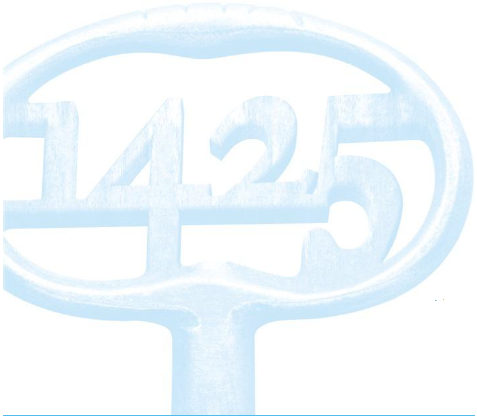
\includegraphics[width=0.2\textwidth]{../LaTeX/Figures/Picture2.png}
	\caption{Example figure}
\end{figure}





%Bijlagen
\begin{appendices}
\chapter{Title of appendix}
Add Appendix here.


\end{appendices}




%Bibiografie
\clearpage
\bibliographystyle{agsm}
%you have to add the bibliography items in mijnbibliografie.bib. Most editors offer a menu for this. Also, in google scholar (settings, advanced) you can turn on @get bibtex citation@, this gives you a text to copy in the bibfile.

\bibliography{../LaTeX/bibliografie} 
\addcontentsline{toc}{chapter}{Bibliography}

\vfill


%Eind
\newpage
\thispagestyle{empty}
\newgeometry{textwidth=540pt,textheight=780pt,top=20pt,left=20pt,right=20pt}
\begin{figure}[ht]
\begin{flushright}

\includegraphics[width=0.5\textwidth]{../LaTeX/Layout/Picture3.png}	
\end{flushright}
\end{figure}
\vfill
\begin{picture}(550,40)
\put(0,0){\colorbox{kuleuven}{\makebox(520,52){}}}
\end{picture}

\end{document}